\documentclass[10pt,mathserif]{beamer}

\usepackage{graphicx,amsmath,amssymb,psfrag,mathtools}
\usepackage{soul}
\usepackage{amsmath,amsfonts,amsthm,bbm}
\usepackage{stmaryrd}
\usepackage{subcaption}



%Code block environment
\usepackage{listings}


\definecolor{lightgrey}{gray}{0.8}
\definecolor{medgrey}{gray}{0.6}
\definecolor{darkgrey}{gray}{0.4}
\usepackage{xcolor}
\lstset { %
    backgroundcolor=\color{black!5}, % set backgroundcolor
    basicstyle=\ttfamily,
    showstringspaces=false,
    commentstyle = \ttfamily,
    commentstyle=\color{commentgreen}\ttfamily,
    morecomment=[l][\color{darkgrey}]{//},
}



\usepackage{tikz}
\usetikzlibrary{matrix,chains,positioning,decorations.pathreplacing,arrows}
\usetikzlibrary{positioning,calc}
\usepackage{tkz-euclide}
%\usetkzobj{all}





%-------------------------------------------------------------------------------
%Definition of operator font
 \usepackage[bb=boondox]{mathalfa}
%% import \varmathbb without affecting other fonts
\usepackage{xparse}
\DeclareFontFamily{U}{ntxmia}{}
\DeclareFontShape{U}{ntxmia}{m}{it}{<-> ntxmia }{}
\DeclareFontShape{U}{ntxmia}{b}{it}{<-> ntxbmia }{}
\DeclareSymbolFont{lettersA}{U}{ntxmia}{m}{it}
\SetSymbolFont{lettersA}{bold}{U}{ntxmia}{b}{it}
\ExplSyntaxOn
\NewDocumentCommand{\varmathbb}{m}
 {
  \tl_map_inline:nn { #1 }
   {
    \use:c { varbb##1 }
   }
 }
\tl_map_inline:nn { ABCDEFGHIJKLMNOPQRSTUVWXYZ }
 {
  \exp_args:Nc \DeclareMathSymbol{varbb#1}{\mathord}{lettersA}{\int_eval:n { `#1+67 }}
 }
\exp_args:Nc \DeclareMathSymbol{varbbk}{\mathord}{lettersA}{169}
\ExplSyntaxOff
%%
\makeatletter
\DeclareFontFamily{U}{tipa}{}
\DeclareFontShape{U}{tipa}{m}{n}{<->tipa10}{}
\newcommand{\arc@char}{{\usefont{U}{tipa}{m}{n}\symbol{62}}}%

\newcommand{\arc}[1]{\mathpalette\arc@arc{#1}}

\newcommand{\arc@arc}[2]{%
  \sbox0{$\m@th#1#2$}%
  \vbox{
    \hbox{\resizebox{\wd0}{\height}{\arc@char}}
    \nointerlineskip
    \box0
  }%
}
\makeatother
\newcommand{\opA}{{\varmathbb{A}}}
\newcommand{\opB}{{\varmathbb{B}}}
\newcommand{\opC}{{\varmathbb{C}}}
\newcommand{\opD}{{\varmathbb{D}}}
\newcommand{\opE}{{\varmathbb{E}}}
\newcommand{\opF}{{\varmathbb{F}}}
\newcommand{\opG}{{\varmathbb{G}}}
\newcommand{\opH}{{\varmathbb{H}}}
\newcommand{\opI}{{\varmathbb{I}}}
\newcommand{\opJ}{{\varmathbb{J}}}
\newcommand{\opK}{{\varmathbb{K}}}
\newcommand{\opL}{{\varmathbb{L}}}
\newcommand{\opM}{{\varmathbb{M}}}
\newcommand{\opN}{{\varmathbb{N}}}
\newcommand{\opO}{{\varmathbb{O}}}
\newcommand{\opP}{{\varmathbb{P}}}
\newcommand{\opQ}{{\varmathbb{Q}}}
\newcommand{\opR}{{\varmathbb{R}}}
\newcommand{\opS}{{\varmathbb{S}}}
\newcommand{\opT}{{\varmathbb{T}}}
\newcommand{\opU}{{\varmathbb{U}}}
\newcommand{\opV}{{\varmathbb{V}}}
\newcommand{\opW}{{\varmathbb{W}}}
\newcommand{\opX}{{\varmathbb{X}}}
\newcommand{\opY}{{\varmathbb{Y}}}
\newcommand{\opZ}{{\varmathbb{Z}}}
\newcommand{\opZer}{\mathbb{0}}
%-------------------------------------------------------------------------------



%-------------------------------------------------------------------------------
%Definition of other font types
\newcommand{\va}{{\mathbf{a}}}
\newcommand{\vb}{{\mathbf{b}}}
\newcommand{\vc}{{\mathbf{c}}}
\newcommand{\vd}{{\mathbf{d}}}
\newcommand{\ve}{{\mathbf{e}}}
\newcommand{\vf}{{\mathbf{f}}}
\newcommand{\vg}{{\mathbf{g}}}
\newcommand{\vh}{{\mathbf{h}}}
\newcommand{\vi}{{\mathbf{i}}}
\newcommand{\vj}{{\mathbf{j}}}
\newcommand{\vk}{{\mathbf{k}}}
\newcommand{\vl}{{\mathbf{l}}}
\newcommand{\vm}{{\mathbf{m}}}
\newcommand{\vn}{{\mathbf{n}}}
\newcommand{\vo}{{\mathbf{o}}}
\newcommand{\vp}{{\mathbf{p}}}
\newcommand{\vq}{{\mathbf{q}}}
\newcommand{\vr}{{\mathbf{r}}}
\newcommand{\vs}{{\mathbf{s}}}
\newcommand{\vt}{{\mathbf{t}}}
\newcommand{\vu}{{\mathbf{u}}}
\newcommand{\vv}{{\mathbf{v}}}
\newcommand{\vw}{{\mathbf{w}}}
\newcommand{\vx}{{\mathbf{x}}}
\newcommand{\vy}{{\mathbf{y}}}
\newcommand{\vz}{{\mathbf{z}}}

\newcommand{\vA}{{\mathbf{A}}}
\newcommand{\vB}{{\mathbf{B}}}
\newcommand{\vC}{{\mathbf{C}}}
\newcommand{\vD}{{\mathbf{D}}}
\newcommand{\vE}{{\mathbf{E}}}
\newcommand{\vF}{{\mathbf{F}}}
\newcommand{\vG}{{\mathbf{G}}}
\newcommand{\vH}{{\mathbf{H}}}
\newcommand{\vI}{{\mathbf{I}}}
\newcommand{\vJ}{{\mathbf{J}}}
\newcommand{\vK}{{\mathbf{K}}}
\newcommand{\vL}{{\mathbf{L}}}
\newcommand{\vM}{{\mathbf{M}}}
\newcommand{\vN}{{\mathbf{N}}}
\newcommand{\vO}{{\mathbf{O}}}
\newcommand{\vP}{{\mathbf{P}}}
\newcommand{\vQ}{{\mathbf{Q}}}
\newcommand{\vR}{{\mathbf{R}}}
\newcommand{\vS}{{\mathbf{S}}}
\newcommand{\vT}{{\mathbf{T}}}
\newcommand{\vU}{{\mathbf{U}}}
\newcommand{\vV}{{\mathbf{V}}}
\newcommand{\vW}{{\mathbf{W}}}
\newcommand{\vX}{{\mathbf{X}}}
\newcommand{\vY}{{\mathbf{Y}}}
\newcommand{\vZ}{{\mathbf{Z}}}

\newcommand{\cA}{{\mathcal{A}}}
\newcommand{\cB}{{\mathcal{B}}}
\newcommand{\cC}{{\mathcal{C}}}
\newcommand{\cD}{{\mathcal{D}}}
\newcommand{\cE}{{\mathcal{E}}}
\newcommand{\cF}{{\mathcal{F}}}
\newcommand{\cG}{{\mathcal{G}}}
\newcommand{\cH}{{\mathcal{H}}}
\newcommand{\cI}{{\mathcal{I}}}
\newcommand{\cJ}{{\mathcal{J}}}
\newcommand{\cK}{{\mathcal{K}}}
\newcommand{\cL}{{\mathcal{L}}}
\newcommand{\cM}{{\mathcal{M}}}
\newcommand{\cN}{{\mathcal{N}}}
\newcommand{\cO}{{\mathcal{O}}}
\newcommand{\cP}{{\mathcal{P}}}
\newcommand{\cQ}{{\mathcal{Q}}}
\newcommand{\cR}{{\mathcal{R}}}
\newcommand{\cS}{{\mathcal{S}}}
\newcommand{\cT}{{\mathcal{T}}}
\newcommand{\cU}{{\mathcal{U}}}
\newcommand{\cV}{{\mathcal{V}}}
\newcommand{\cW}{{\mathcal{W}}}
\newcommand{\cX}{{\mathcal{X}}}
\newcommand{\cY}{{\mathcal{Y}}}
\newcommand{\cZ}{{\mathcal{Z}}}
%-------------------------------------------------------------------------------




%-------------------------------------------------------------------------------
%% macros for math notions and operators
\newcommand{\EE}{{\mathbb{E}}}
\newcommand{\expec}{\mathbb{E}}
\newcommand{\Prob}{{\mathrm{Prob}}} % probability

\newcommand{\reals}{\mathbb{R}}
\newcommand{\RR}{\mathbb{R}}
\newcommand{\complex}{\mathbb{C}}
\newcommand{\CC}{\mathbb{C}}
\newcommand{\nats}{\mathbb{N}}
\newcommand{\NN}{\mathbb{N}}
\newcommand{\ZZ}{\mathbb{Z}}
\newcommand{\bigO}{\mathcal{O}}
\newcommand{\order}[1]{{\mathcal{O}\left(#1\right)}}
\renewcommand{\SS}{{\mathbb{S}}}
\newcommand{\SSp}{\mathbb{S}_{+}}
\newcommand{\SSpp}{\mathbb{S}_{++}}
\newcommand{\sign}{\mathrm{sign}}
\newcommand{\vzero}{\mathbf{0}}
\newcommand{\vone}{{\mathbf{1}}}

\renewcommand{\Re}{\operatorname{Re}} 	%Real part
\renewcommand{\Im}{\operatorname{Im}}	%imaginary part

%\newcommand{\supp}{{\mathrm{supp}}} % support
\newcommand{\range}{\mathrm{range}\,} % domain
\newcommand{\tr}{{\mathrm{tr}}} % trace
%-------------------------------------------------------------------------------





%-------------------------------------------------------------------------------
%% Theorem definitions
\setbeamertemplate{theorems}[ams style] 
\newtheorem*{theorem*}{Theorem}
%\newtheorem{lemma}{Lemma}    % already provided by amsthm
\newtheorem{proposition}{Proposition}
%\newtheorem{proof}{Proof}  % already provided by amsthm


%-------------------------------------------------------------------------------
%% operator and convex analysis definitions

\newcommand*{\fix}{\mathrm{Fix}\,}
\newcommand*{\zer}{\mathrm{Zer}\,}
\newcommand*{\gra}{\mathrm{Gra}\,}
\newcommand{\prox}{\mathrm{Prox}}
\newcommand{\proj}{\Pi}
\newcommand{\aff}{\mathrm{aff}\,}    %affine hull
\newcommand{\intr}{\mathrm{int}\,}   %interior
\newcommand{\relint}{\mathrm{ri}\,}  %relative interior
\newcommand{\dom}{\mathrm{dom}\,} % domain
\newcommand{\epi}{\mathrm{epi}\,} % epigraph
\newcommand{\dist}{\mathrm{dist}}
\newcommand{\lagrange}{\mathbf{L}}  %saddle function
\newcommand{\fitzpatrick}{\mathbf{F}}   %Fitzpatrick function
\newcommand{\vecdelay}{\boldsymbol{d}}   %vector delay
\DeclareMathOperator*{\argmin}{argmin}
\DeclareMathOperator*{\argmax}{argmax}

%-------------------------------------------------------------------------------
%SRG definitions
\newcommand{\ereal}{\overline{\mathbb{R}^2}}
\newcommand{\ecomplex}{\overline{\mathbb{C}}}
\newcommand{\binfty}{{\boldsymbol \infty}}
\newcommand{\rarc}{\mathrm{Arc}^+}
\newcommand{\larc}{\mathrm{Arc}^-}


%-------------------------------------------------------------------------------




%-------------------------------------------------------------------------------
%Miscellaneous Stuff
%% sequences
\newcommand{\itom}{_{i=1}^{m}}
\newcommand{\ieqm}{i=1,\dots,m}

% use \numberthis to add an equation number in align*
\newcommand\numberthis{\addtocounter{equation}{1}\tag{\theequation}}

\newcolumntype{P}[1]{>{\centering\arraybackslash}p{#1}}

\mode<presentation>
{
\usetheme{default}
}
\setbeamertemplate{navigation symbols}{}
\usecolortheme[rgb={0.13,0.28,0.59}]{structure}
\setbeamertemplate{itemize subitem}{--}
\setbeamertemplate{frametitle} {
	\begin{center}
	  {\large\bf \insertframetitle}
	\end{center}
}

\newcommand\footlineon{
  \setbeamertemplate{footline} {
    \begin{beamercolorbox}[ht=2.5ex,dp=1.125ex,leftskip=.8cm,rightskip=.6cm]{structure}
      \footnotesize \insertsection
      \hfill
      {\insertframenumber}
    \end{beamercolorbox}
    \vskip 0.45cm
  }
}
\footlineon


\newcommand\footlineoff{
  \setbeamertemplate{footline} {
    \begin{beamercolorbox}[ht=2.5ex,dp=1.125ex,leftskip=.8cm,rightskip=.6cm]{structure}
      \footnotesize 
      \hfill
      {\insertframenumber}
    \end{beamercolorbox}
    \vskip 0.45cm
  }
}


\newcommand\blfootnote[1]{%
  \begingroup
  \renewcommand\thefootnote{}\footnote{#1}%
  \addtocounter{footnote}{-1}%
  \endgroup
}


\AtBeginSection[] 
{ 
	\begin{frame}<beamer> 
		\frametitle{Outline} 
		\tableofcontents[currentsection,currentsubsection] 
	\end{frame} 
} 

%% wotao's preference

        % itemize, black bullet, %150 spacing between items using "witemize"
        \newenvironment{witemize}{\itemize\addtolength{\itemsep}{0.3\baselineskip}}{\enditemize}

\iffalse
        % \setbeamertemplate{itemize items}[square]
        \setbeamertemplate{itemize items}{\textbullet}
        \setbeamercolor{itemize item}{fg=black}
        \setbeamercolor{itemize subitem}{fg=black}
        \setbeamercolor{itemize subsubitem}{fg=black}
        \setbeamercolor{enumerate item}{fg=black}
        \setbeamercolor{enumerate subitem}{fg=black}
        \setbeamercolor{enumerate subsubitem}{fg=black}
        \setbeamertemplate{itemize/enumerate body begin}{\normalsize}
        \setbeamertemplate{itemize/enumerate subbody begin}{\normalsize}
        \setbeamertemplate{itemize/enumerate subsubbody begin}{\normalsize}

        % itemize enumerate use normal sized texts
        \setbeamertemplate{itemize/enumerate body begin}{\normalsize}
        \setbeamertemplate{itemize/enumerate subbody begin}{\normalsize}
        \setbeamertemplate{itemize/enumerate subsubbody begin}{\normalsize}

        % block, black over gray with no shadow
        \setbeamertemplate{blocks}[rounded][shadow=false]
        \setbeamercolor{block title}{fg=black,bg=gray!40}
        \setbeamercolor{block body}{fg=black,bg=gray!10}
\fi

\author{Ernest K. Ryu and Wotao Yin}

\date{Large-Scale Convex Optimization via Monotone Operators}


\title{\large \bfseries Parallel Computing}

\begin{document}

\frame{
\thispagestyle{empty}
\titlepage
}

\begin{frame}
\frametitle{Computational complexity and parallel computing}

Briefly discuss computational complexity. 
\vspace{0.2in}

Use examples to introduce parallel algorithms. 
%The notion of computational complexity we consider is, in a sense, incomplete as it only accounts for the cost of arithmetic operations, while ignoring other costs such as the cost of coordination and communication between computational agents.
%\vspace{0.2in}

%Useful for approximately analyzing run time of algorithms.
\end{frame}


\section{Computational complexity via flop count}

\begin{frame}
\frametitle{Floating-point operations}
A floating-point operation (flop) is a single arithmetic operation on a floating-point number or a pair of those numbers such as addition, subtraction, multiplication, and division.

\vspace{0.2in}
For simplicity, we also count a non-elementary function such as $\exp{}$, $\log{}$, or $\sqrt{~}$ as a single flop.

\vspace{0.2in}\pause
For example, given $x\in \reals^n$,
\[
\|x\|=\sqrt{x_1^2+\dots+x_n^2}
\]
costs $2n=\order{n}$ flops to compute. \\
($n$ multiplications, $n-1$ additions, and $1$ square root.)
\end{frame}



\begin{frame}
\frametitle{Floating-point operations}
\begin{itemize}
\item
$Ax$ costs $\order{mn}$ flops, where $A\in \reals^{m\times n}$ and $x\in \reals^n$.
\item
$AB$ costs $\order{mnp}$ flops, where $A\in \reals^{m\times n}$ and $B\in \reals^{n\times p}$.
\item
For $ABx$, use  $A(Bx)$, costing $\order{mn+np}$, instead of $(AB)x$, costing $\order{mnp}$,
 where $A\in \reals^{m\times n}$, $B\in \reals^{n\times p}$, and $x\in \reals^{p}$.
\item
$A^{-1}$ costs $\order{n^3}$, where $A\in \reals^{n\times n}$.
\end{itemize}
% We expect
% This means matrix-vector products of
% matrix inverses of $1000\times 1000$ matrices takes $1$ second to compute.
\end{frame}

\begin{frame}{Processing power in flops}

\emph{Flop per second} is an indicator of the processing power of (a core of) of a CPU/GPU.
\vspace{0.2in}

Each CPU core can process roughly $10^9$ flops per second.
\vspace{0.2in}\pause

(flops needed)/(flops offered) roughly predicts the run time of an algorithm on a CPU.
But this is a very rough estimate; expect a 10-fold or even a 100-fold inaccuracy.
\end{frame}


\begin{frame}
\frametitle{Algorithm vs.\ method}
Algorithm and method both specify how to compute a quantity of interest.\\
\medskip
But, they sit at different levels of specifications.
\medskip\pause

Difference:
\begin{itemize}
\item
method is a higher-level description expressed in mathematical equations 
\item
algorithm is a step-by-step procedure unambiguously describing the steps the computer takes
\end{itemize}
%Although this distinction is not precise, it is useful.
\pause
If an algorithm carries out the idea described by a method, we say the algorithm implements the method.
\end{frame}


\begin{frame}[plain]
\frametitle{Algorithm vs.\ method}
In a rigorous discussion, flop count is ascribed to algorithm, not method.
\vspace{0.2in}\pause

Example: consider $A\in \reals^{m\times n}$, $b\in \reals^m$, and the method
\[
x^{k+1}=x^k-\alpha A^\intercal(Ax^k-b).
\]

Algorithm corresponding to 
\[
A^\intercal(Ax^k-b)
\]
costs $\order{mn}$ flops per iteration. But, by precomputing and storing $A^\intercal A\in\reals^{n\times n}$ and $A^\intercal b\in \reals^m$, algorithm corresponding to 
\[
(A^\intercal A)x^k-A^\intercal b
\]
costs $\order{n^2}$ flops per iteration.

% \vspace{0.2in}\pause
% Often more than one way to implement a method.
% When implementation clear from the context, informally ascribe the flop count to the method.
\end{frame}


\begin{frame}[fragile]
\frametitle{Flop-count operator}
Define: flop-count operator
\[
\mathcal{F}\left[\{x_1,\dots,x_n\}\mapsto\{y_1,\dots,y_m\}\,|\,\mathcal{A}\right]:
\]
number of flops $\mathcal{A}$ to compute $\{y_1,\dots,y_m\}$ given $\{x_1,\dots,x_n\}$.
(Algorithm $\mathcal{A}$, not a method, that determines the flop count.)
\medskip
When $\mathcal{A}$ is clear from context, %omit $\mathcal{A}$
% and 
write
$
\mathcal{F}\left[\{x_1,\dots,x_n\}\mapsto\{y_1,\dots,y_m\}\right].
$
%When the input and/or output is a single quantity, we omit the curly braces and write
%\[
%\mathcal{F}[x\mapsto y].
%\]
%\vspace{0.2in}
%
%For example, we write
%\[
%\mathcal{F}[x\mapsto\|x\|]=2n=\order{n}.
%\]
%and
\medskip \pause
For example, when $A\in \reals^{m\times n}$
\begingroup\makeatletter\def\f@size{9}\check@mathfonts
\begin{align*}
\mathcal{F}[A\mapsto(I+\alpha A^\intercal A)^{-1}]
&=
\mathcal{F}[A\mapsto I+\alpha A^\intercal A]+\mathcal{F}[ I+\alpha A^\intercal A\mapsto (I+\alpha A^\intercal A)^{-1}]\\
&=\order{mn^2}+\order{n^3}
=\order{(m+n)n^2}.
\end{align*}
\endgroup
\end{frame}


\begin{frame}[fragile,plain]
\frametitle{Flop-count operator}
As another example, consider
\[
\begin{array}{ll}
\underset{x\in \reals^n}{\mbox{minimize}}
&
\displaystyle{\frac{1}{2}\|Ax-b\|^2+\lambda\|x\|_1,}
\end{array}
\]
where $A\in \reals^{m\times n}$, $b\in \reals^m$, and $\lambda>0$. DRS is
%\S\ref{ss:methods}
\begin{align*}
x^{k+1/2}&=(I+\alpha A^\intercal A)^{-1}(z^k+\alpha A^\intercal b)\\
x^{k+1}&=S(2x^{k+1/2}-z^k;\alpha \lambda)\\
z^{k+1}&=z^k+x^{k+1}-x^{k+1/2},
\end{align*}
where $S$ is soft-thresholding.
 \pause
A naive implementation costs
\begingroup\makeatletter\def\f@size{9}\check@mathfonts
\begin{align*}
\mathcal{F}\left[z^k\mapsto z^{k+1}\right]&=
\mathcal{F}\left[A\mapsto (I+\alpha A^\intercal A)^{-1}\right]
+
\mathcal{F}\left[\{z^k,(I+\alpha A^\intercal A)^{-1},A,b\}\mapsto x^{k+1/2}\right]\\
&\quad +
\mathcal{F}\left[\{x^{k+1/2},z^k\}\mapsto x^{k+1}\right]
+
\mathcal{F}\left[\{z^k,x^{k+1/2},x^{k+1}\}\mapsto z^{k+1}\right]\\
&=\order{(m+n)n^2}+\order{(m+n)n}
+\order{n}+\order{n}\\
&=\order{(m+n)n^2}.
\end{align*}
\endgroup
\end{frame}




\begin{frame}
\frametitle{Flop-count operator}
Reduce this cost.
When $m\ge n$, precompute $(I+\alpha A^\intercal A)^{-1}$ with cost
\[
\mathcal{F}\left[
A\mapsto (I+\alpha A^\intercal A)^{-1}
\right]=\order{mn^2}
\]
and $\alpha A^\intercal b$ with cost
\[
\mathcal{F}\left[
\{\alpha, A,b\}\mapsto \alpha A^\intercal b
\right]=\order{mn}.
\]
\pause 
In subsequent iterations,
\begin{align*}
\mathcal{F}&\left[\{z^k,(I+\alpha A^\intercal A)^{-1},\alpha A^\intercal b\}\mapsto z^{k+1}\right]\\&=
\mathcal{F}\left[\{z^k,(I+\alpha A^\intercal A)^{-1},\alpha A^\intercal b\}\mapsto x^{k+1/2}\right]
+
\mathcal{F}\left[\{x^{k+1/2},z^k\}\mapsto x^{k+1}\right]\\
&\quad+
\mathcal{F}\left[\{z^k,x^{k+1/2},x^{k+1}\}\mapsto z^{k+1}\right]\\
&=\order{n^2}
+\order{n}+\order{n}\\
&=\order{n^2}.
\end{align*}
% See Exercise~\ref{exercise:chol} for further discussion on the Cholesky factorization.
%When $m\le n$, we can use the matrix inverse lemma. See Exercise~\ref{exercise:woodbury}.
\end{frame}






\section{Parallel computing}
\begin{frame}[fragile]
\frametitle{Simplified view of parallel computing}
(Over)simplified view of parallel computing: a group of computational agents working \emph{simultaneously} on the same task.
\medskip

Example of agents: CPU cores, GPU cores, or computers connected via LAN or over the internet.
%\medskip

%Not all computational tasks can benefit from parallel computing.
%Those with algorithms that can significantly speed up on multiple agents are called \emph{parallelizable}.

\vspace{0.2in}\pause


If $p$ processors, $A,B\in \reals^{m\times n}$, and $p\le mn$, then $C=A+B$ requires $\order{mn/p}$ flops for each processor:
\begin{lstlisting}
parallel for i=1,...,m, j=1,...,n {
  C[i,j] = A[i,j]+B[i,j]
}
\end{lstlisting}
%The ``parallel for'' loop represents $mn$ independent tasks.
%If $p$ divides $mn$, then each of the $p$ processors can perform exactly $mn/p$ out of the $mn$ tasks.
%Otherwise, partition the $mn$ tasks into $p$ groups of sizes roughly equal to $mn/p$ and assign them to the $p$ processors.
\end{frame}

\begin{frame}[fragile]
\frametitle{Embarrassingly parallel}
A task is embarrassingly parallel if trivial to parallelize.\\
(The fact that little effort is needed is ``embarrassing.'')
\vspace{0.2in}\pause

For example, $v=Ax$ is embarrassingly parallel:
\begin{lstlisting}
parallel for i=1,...,m {
  v[i] = 0;
  for j=1,...,n 
    v[i] += A[i,j]*x[j]
}
\end{lstlisting}
\end{frame}

\begin{frame}
\frametitle{Not everything is parallelizable}
% The multiplication $A$ can be parallelized. Assuming $p\ll m$ and $p\ll n$, then the whole thing can be done in $\order{mn/p}$ time.
Some tasks are difficult to parallelize.
Consider DRS:
\begin{align*}
x^{k+1/2}&=\prox_{\alpha f}(z^k)\\
x^{k+1}&=\prox_{\alpha g}(2x^{k+1/2}-z^k)\\
z^{k+1}&=z^k+x^{k+1}-x^{k+1/2}.
\end{align*}
The three steps must be computed serially.
 

%When we have $p\le n$ processors, the vector sum $z^k+x^{k+1}-x^{k+1/2}$ can be split up into $p$ independent parts each costing $\order{n/p}$ flops.

\vspace{0.2in}
Computational bottleneck usually in $\prox_{\alpha f}$ or $\prox_{\alpha g}$.
If the bottleneck step (or steps) is not parallelizable by itself, DRS is not parallelizable.
\end{frame}





\begin{frame}
\frametitle{Parallel flop count operator}
Assume $\mathcal{A}$ has access to $p$ processors.\\
(But, $\mathcal{A}$ may or may not process $p$ flops in each parallel step.)
%In some steps, $\mathcal{A}$ may be unable to fully utilize the $p$ computing units and will process fewer than $p$ flops.
\vspace{0.2in}


Notation: parallel flop-count operator:
\[
\mathcal{F}_p\left[\{x_1,\dots,x_n\}\mapsto\{y_1,\dots,y_m\}\,|\,\mathcal{A}\right]
\]
the \emph{number of parallel steps} that algorithm $\mathcal{A}$ takes to compute $\{y_1,\dots,y_m\}$ given $\{x_1,\dots,x_n\}$ and $p$ processors.
%As before, we omit the dependency on $\mathcal{A}$ if the algorithm is clear from context, and we omit the curly braces when the input and/or output is a single quantity.
\end{frame}



\begin{frame}[plain]
\frametitle{Parallelizable methods and operators}
An algorithm is parallel if it utilizes multiple computing units and is serial otherwise.\pause

But, A method is parallelizable if it has an parallel algorithm to provide a significant speedup.
%(``Significant'' depends on context.)
%We say an operator is parellelizable if there is a parallelizable method for evaluating it.

\vspace{0.2in}\pause
Computing $\{y_1,\dots,y_m\}$ given $\{x_1,\dots,x_n\}$ is parallelizable if
\[
\mathcal{F}_p\left[\{x_1,\dots,x_n\}\mapsto\{y_1,\dots,y_m\}\right]
\ll
\mathcal{F}\left[\{x_1,\dots,x_n\}\mapsto\{y_1,\dots,y_m\}\right]
\]
for large enough $p$.
Meaning of $\ll$ depends on context. \pause If
\[
\mathcal{F}_p\left[\{x_1,\dots,x_n\}\mapsto\{y_1,\dots,y_m\}\right]
\sim \frac{C}{p}
\mathcal{F}\left[\{x_1,\dots,x_n\}\mapsto\{y_1,\dots,y_m\}\right]
\]
for some $C>0$ not too large, then parallelizable.

\vspace{0.2in}\pause
Operator $\opT$ is parallelizable if
$
\mathcal{F}_p\left[x\mapsto \opT x\right]
\ll
\mathcal{F}\left[x\mapsto \opT x\right].
$

\end{frame}

\begin{frame}[fragile]
\frametitle{Reduction}
Reduction combines a set of numbers into one with an associative binary operator.

\vspace{0.2in}\pause
A common example is the sum
\[
    x_\mathrm{sum} = \sum_{i=1}^nx_i,
\]
where $x_1,\dots,x_n\in\reals$.
With $p=1$ processor, reduction costs $\order{n}$.
    % \qquad
    % x_\mathrm{min} = \min\{x_1,\dots,x_n\},
    % \qquad
    % x_\mathrm{max} = \max\{x_1,\dots,x_n\},
\end{frame}



\begin{frame}[fragile,plain]
\frametitle{Parallel reduction}
With $p\ge \lfloor n/2 \rfloor$ processors, reduction takes $\order{\log n }$ steps.
In the following example with $n=8$ and $p=4$, $\cF_p\left[\{x_1,\dots,x_8\}\mapsto x_\mathrm{sum}\right]=3$.
\vspace{0.1in}

\raisebox{-.5\height}{
\!\!\!\!\!\!\!\!\!\!\!\!
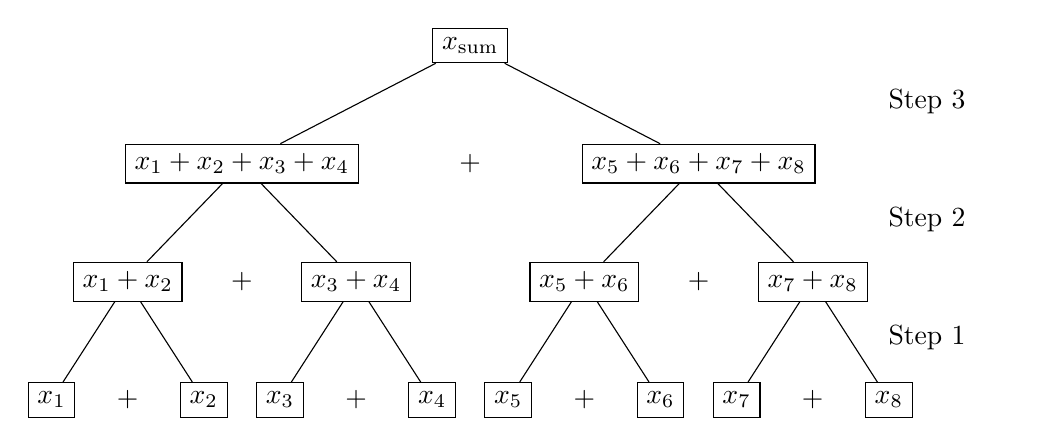
\begin{tikzpicture}[level/.style={sibling distance=58mm/#1}]
\node [rectangle,draw] (z){$x_\mathrm{sum}$}
  child {node [rectangle,draw] (a) {$x_1+x_2+x_3+x_4$}
    child {node [rectangle,draw] (b) {$x_1+x_2$}
      child {node [rectangle,draw] (c) {$x_1$}}
      child {node [rectangle,draw] (d) {$x_2$}}
    }
    child {node [rectangle,draw] (e) {$x_3+x_4$}
      child {node [rectangle,draw] (f) {$x_3$}}
      child {node [rectangle,draw] (g) {$x_4$}}
    }
  }
  child {node [rectangle,draw] (h) {$x_5+x_6+x_7+x_8$}
    child {node [rectangle,draw] (i) {$x_5+x_6$}
      child {node [rectangle,draw] (j) {$x_5$}}
      child {node [rectangle,draw] (k) {$x_6$}}
    }
  child {node [rectangle,draw] (l) {$x_7+x_8$}
      child {node [rectangle,draw] (m) {$x_7$}}
      child {node [rectangle,draw] (n) {$x_8$}
        child [grow=right] {node  {} edge from parent[draw=none]
          child [grow=up] {node[below=0.17in] {\hspace{-0.8in}Step 1} edge from parent[draw=none]
            child [grow=up] {node  {\hspace{-0.8in}Step 2} edge from parent[draw=none]
              child [grow=up] {node  {\hspace{-0.8in}Step 3} edge from parent[draw=none]}
            }
          }
        }
      }
  }
};
\path (a) -- (h) node [midway] {$+$};
\path (b) -- (e) node [midway] {$+$};
\path (i) -- (l) node [midway] {$+$};
\path (c) -- (d) node [midway] {$+$};
\path (f) -- (g) node [midway] {$+$};
\path (j) -- (k) node [midway] {$+$};
\path (m) -- (n) node [midway] {$+$};
\end{tikzpicture}
}
\vspace{0.1in}

General strategy: follow a binary tree with depth $\log_2 n$.
\end{frame}



\begin{frame}[fragile,plain]
\frametitle{Parallel reduction}
With $p< \lfloor n/2 \rfloor$ processors, reduction takes $\order{n/p+\log p }$ steps.
In the following example with  $n=40$ and $p=4$, $\cF_p\left[\{x_1,\dots,x_{40}\}\mapsto x_\mathrm{sum}\right]=40/4 - 1 + \log_2 4 =11$.

\vspace{0.1in}

\raisebox{-.5\height}{
\!\!\!\!\!\!\!\!\!\!\!\!\!\!\!
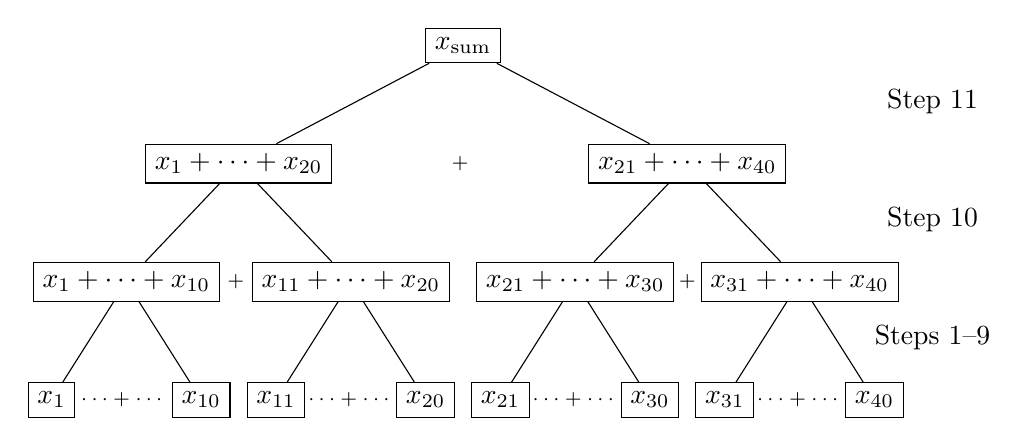
\begin{tikzpicture}[level/.style={sibling distance=57mm/#1}]
\node [rectangle,draw] (z){$x_\mathrm{sum}$}
  child {node [rectangle,draw] (a) {$x_1+\dots+x_{20}$}
    child {node [rectangle,draw] (b) {$x_1+\dots+x_{10}$}
      child {node [rectangle,draw] (c) {$x_1$}}
      child {node [rectangle,draw] (d) {$x_{10}$}}
    }
    child {node [rectangle,draw] (e) {$x_{11}+\dots+x_{20}$}
      child {node [rectangle,draw] (f) {$x_{11}$}}
      child {node [rectangle,draw] (g) {$x_{20}$}}
    }
  }
  child {node [rectangle,draw] (h) {$x_{21}+\dots+x_{40}$}
    child {node [rectangle,draw] (i) {$x_{21}+\dots+x_{30}$}
      child {node [rectangle,draw] (j) {$x_{21}$}}
      child {node [rectangle,draw] (k) {$x_{30}$}}
    }
  child {node [rectangle,draw] (l) {$x_{31}+\dots+x_{40}$}
      child {node [rectangle,draw] (m) {$x_{31}$}}
      child {node [rectangle,draw] (n) {$x_{40}$}
        child [grow=right] {node  {} edge from parent[draw=none]
          child [grow=up] {node[below=0.17in]  {\hspace{-0.6in}Steps 1--9} edge from parent[draw=none]
            child [grow=up] {node  {\hspace{-0.6in}Step 10} edge from parent[draw=none]
              child [grow=up] {node  {\hspace{-0.6in}Step 11} edge from parent[draw=none]}
            }
          }
        }
      }
  }
};
\path (a) -- (h) node [midway,font=\scriptsize] {$+$};
\path (b) -- (e) node [midway,font=\scriptsize] {$+$};
\path (i) -- (l) node [midway,font=\scriptsize] {$+$};
\path (c) -- (d) node [midway,font=\scriptsize] {$\cdots+\cdots$};
\path (f) -- (g) node [midway,font=\scriptsize] {$\cdots+\cdots$};
\path (j) -- (k) node [midway,font=\scriptsize] {$\cdots+\cdots$};
\path (m) -- (n) node [midway,font=\scriptsize] {$\cdots+\cdots$};
\end{tikzpicture}}
\vspace{0.1in}

General strategy: (i) partition $n$ numbers into $p$ groups of sizes roughly $n/p$,
(ii) reduce within $p$ groups with $\order{n/p}$ steps, (iii) reduce $p$ numbers with $\order{\log p}$ steps.
\end{frame}

\begin{frame}
\frametitle{Parallel reduction}
To summarize,
\begin{align*}
  \mathcal{F}_p\left[\{x_1,\ldots,x_n\}\mapsto x_\mathrm{sum}\right] =
  \begin{cases}
    \order{n} & \mbox{if } p = 1 \\
    \order{n/p + \log p} & \mbox{if } 1< p < \lfloor n/2 \rfloor \\
    \order{\log n} & \text{if } p \ge \lfloor n/2 \rfloor .
  \end{cases}
\end{align*}
%We combine the cases to
%\[
%%\label{eq:reduce_flops}
%\mathcal{F}_p\left[\{x_1,\ldots,x_n\}\mapsto x_\mathrm{sum}\right] =\order{n/p + \log p}
%\quad\text{ for }p\le n/2.
%\]

%Recall that the $\cO$-notation is an upper bound. When $p\gg n$, the bound is not tight but still valid.

%\eqref{eq:reduce_flops} also is the parallel flop count of other reduction operations such as:
\pause
Likewise, we can compute
\begin{itemize}
  \item minimum and maximum of $x_1,\dots,x_n\in\reals$,
  \item arithmetic mean, geometric mean, and product of $x_1,\dots,x_n\in\reals$,
  \item $\langle x,y\rangle$ for $x,y\in\reals^n$, and
  \item $\|x\|_1$ and $\|x\|_\infty$ for $x\in\reals^n$.
\end{itemize}
%with using $\order{m/p + \log p}$ steps for $p\le n/2$.
\end{frame}

\begin{frame}[plain]
\frametitle{Parallel matrix-vector multiplication}
Let $A\in \reals^{m\times n}$ and $x\in \reals^n$ and consider $\{A,x\}\mapsto b$.

\[
\mathcal{F}_p\left[\{A,x\}\mapsto b\right] 
=
\left\{
\begin{array}{ll}
\order{mn}&\text{if }p=1\\
\order{mn/p}&\text{if }p\le m\\
\order{mn /p + \log (p/m)}&m<p< mn/2\\
\order{ \log n}&\text{if } mn/2 \le p.
\end{array}
\right.
\]
%
%With $p=1$,
%\[
%\mathcal{F}_1\left[
%\{A,x\}\mapsto b
%\right]=\order{mn}
%\]
%%With $p=1$ processor, $b=Ax$ requires $\order{mn}$ steps.
%With $p\le m$,
%% processors, $b=Ax$ requires $\order{mn/p}$ steps.
%\[
%\mathcal{F}_p\left[
%\{A,x\}\mapsto b
%\right]=\order{mn/p}
%\]
%With $m<p\le mn/2$,
%% processors, $b=Ax$ requires $\order{mn/p}$ steps.
%\[
%\mathcal{F}_p\left[
%\{A,x\}\mapsto b
%\right]=\order{mn /p + \log (p/m)}
%\]
%With $ mn/2<p$,
%% processors, $b=Ax$ requires $\order{mn/p}$ steps.
%\[
%\mathcal{F}_p\left[
%\{A,x\}\mapsto b
%\right]=\order{ \log (n)}
%\]

For $m<p$, assign $\frac{p}{m}$ processors to compute $b_i = \sum_{j=1}^n A_{i,j}x_j$ with parallel reduction.

%with $\order{n /(p/m) + \log(p/m)}$ steps through 

%To see why, 
%we assign each processor with roughly $m/p$ of the $m$ independent subtasks $b_i = \sum_{j=1}^n A_{i,j}x_j$ for $\ieqm$.
%With $p\ge m$ processors, $b=Ax$ requires $\order{mn /p + \log (p/m)}$ steps.
% with the strategy used for computing parallel reduction.
%We combine the cases to
%\begin{align*}
%  \mathcal{F}_p\left[\{A,x\}\mapsto Ax\right] = \mathcal{O}\left(mn/p + \max\left\{0,\log(p/m)\right\}\right)
%  \quad\text{ for }p\le mn/2.
%\end{align*}

\end{frame}


\begin{frame}
\frametitle{Other costs: coordination and communication}
On a multi-core CPU, counting only flops is a useful approximation. Flops maybe \emph{inadequate} since
\begin{itemize}
    \item data organization is important
    \item latency, data transmission, and coordination may take significant time.
\end{itemize}
\medskip\pause


Parallel computing on a graphics processing unit (GPU) relies on thousands of slower processors.
Cost of coordination may be significant.
%and thus should be taken into account.
\medskip\pause


When going distributed and decentralized, many computers (as opposed to CPU cores on a chip) operate in parallel and communicate.
Cost of communication (latency, transmission, and coordination) becomes more significant.
\end{frame}


\begin{frame}
\frametitle{Parallelizing linear algebra vs.\ high-level parallelism}
When a method relies on linear algebraic operations (like $\{A,x\}\mapsto Ax$), it is possible to parallelize the linear algebra.

\vspace{0.2in}\pause

In some cases,  a method itself is parallelizable at a higher level.

\vspace{0.2in}\pause

There are also cases to run a method with different data; this task is parallelizable at an even higher level.

%\vspace{0.2in}
%
%We discuss several methods for finite-sum minimization problems and to what extent they can be parallelized.
\end{frame}


\begin{frame}[plain]
\frametitle{Example: Sum of smooth functions}
Consider 
\[
\begin{array}{ll}
\underset{x\in \reals^n}{\mbox{minimize}}&
\displaystyle{f(x) + \frac{1}{m}\sum\itom h_i(x),}
\end{array}
\]
where $h_1,\dots,h_m$ are differentiable. \pause FBS is
\begin{align*}
  v^k & = -  \frac{\alpha}{m}\sum\itom \nabla h_i(x^k)\\% &&\text{parallel gradient and sum},\\
%  \overline{y}^k & = \frac{1}{m}\sum\itom  y_i^k &&\text{parallel sum},\\
  x^{k+1} & = \prox_{\alpha f}\left(x^k + v^k\right)% &&\text{parallel vector addition}.
\end{align*}
\pause
Assume $\prox_{\alpha f}$ costs $C_f$ flops and $\nabla h_i$ costs $C_h$ flops (or fewer).
Then
\begin{align*}
\mathcal{F}_p\left[x^k\mapsto x^{k+1}\right]
&=
\mathcal{F}_p\left[x^k\mapsto\{\nabla h_i(x^k)\}\itom  \right]+
\mathcal{F}_p\left[\{\nabla h_i(x^k)\}\itom \mapsto v^k \right]\\
&\qquad\qquad+
\mathcal{F}_p\left[\{x^k,v^k \}\mapsto x^{k+1}\right]\\
% &=\order{mC_h/p} + \order{mn/p + \max\{0,\log(p/m)\}} + \order{\max\{1,n/p\}+C_f}\\
% &=\order{(C_h + n)m/p + \max\{0,\log(p/m)\}+ C_f}.% \numberthis \label{eq:par_fin_sum_fc}
&=\order{mC_h/p} + \order{mn/p } + \order{n/p+C_f}\\
&=\order{(C_h + n)m/p+ C_f}.% \numberthis \label{eq:par_fin_sum_fc}
\end{align*}
 for $p\le \min\{m,n\}$.
Method parallelizable if $C_f=\order{(C_h + n)m/p}$.
\end{frame}


\begin{frame}[plain]
\frametitle{Example: Sum of proximable functions}
Consider
\[
\begin{array}{ll}
\underset{x\in \reals^n}{\mbox{minimize}} & \displaystyle{f(x)+\frac{1}{m}\sum\itom  g_i(x)}.
\end{array}
\]
Using the consensus technique, reformulate  into
\[
%\label{eq:paral_consensus}
\begin{array}{ll}
\underset{x_1,\dots,x_m\in\reals^{n}}{\mbox{minimize}} &
\displaystyle{f(x_1)+\delta_C(x_1,\dots,x_m)+\frac{1}{m}\sum\itom  g_i(x_i),}
%\mbox{subject to} & \vx\in C,
\end{array}
\]
where $C=\{(x_1,\dots,x_m)\,|\,x_1=\dots=x_m\}$.
%and $\vx^{k+1/2}=(x^{k+1/2},\dots,x^{k+1/2})$.
 \pause
DRS is
\begin{align*}
x^{k+1/2} &= \prox_{\alpha f}\left(\frac{1}{m}\sum\itom  z^{k}_i\right),\\
x^{k+1}_i &=\prox_{\alpha g_i}(2x^{k+1/2}-z^k_i)\\
z^{k+1}_i &= z^k_i +  x^{k+1}_i-x^{k+1/2}\qquad\text{for }\ieqm.
\end{align*}
\pause 
Assume $\prox_{\alpha f}$ costs $C_f$ and $\prox_{\alpha g_i}$ costs $C_g$ (or fewer).
%Write $\vz^k=(z_1^k,\dots,z_m^k)$.
For $p\le m$,
\begin{align*}
\mathcal{F}_p\left[\vz^k\mapsto \vz^{k+1}\right]&=
\mathcal{F}_p\left[\vz^k\mapsto x^{k+1/2}\right]+
\mathcal{F}_p\left[\{\vz^k, x^{k+1/2}\}\mapsto \vz^{k+1}\right]\\
% &=
% \order{mn/p + \max\{0,\log(p/m)\}+C_f} +\order{ \max\{1,nm/p\}+C_g\max\{1,m/p\}}\\
%&=\order{mn/p + \max\{0,\log(p/m)\}+C_f+ C_g\max\{1,m/p\}}.
&=\order{mn/p+C_f+ C_gm/p}.
\end{align*}
\end{frame}


\begin{frame}
\frametitle{Example: Sum of proximable functions and a strongly convex function}
Consider primal problem
\[
%\label{eq:par_prox_fin_sum}
\begin{array}{ll}
\underset{x\in \reals^{n}}{\mbox{minimize}}&
\displaystyle{f(x) + \sum\itom g_i(a_i^\intercal x-b_i)}
\end{array}
\]
%This setup arises often in signal processing and machine learning.
and dual problem
\[
%\label{eq:par_prox_fin_sum_dual}
\begin{array}{ll}
\underset{u_1,\ldots,u_m\in\RR}{\mbox{maximize}}&
\displaystyle{-f^*\left(-\sum\itom u_ia_i\right) - \sum\itom( g^*_i(u_i)+b_iu_i)}
\end{array}
\]
generated by
\begin{align*}
  \lagrange(x,u_1,\dots,u_m) = f(x) + \sum\itom  \langle u_i, a_i^\intercal x-b_i\rangle - \sum\itom g^*_i(u_i),
\end{align*}
where $a_1,\dots,a_m\in\reals^n$, $b_1,\dots,b_m\in \reals$, $f$ is a strongly convex CCP function on $\reals^n$, and $g_1,\dots,g_m$ are proximable CCP functions on $\reals$.
\end{frame}

\begin{frame}
\frametitle{Example: Sum of proximable functions and a strongly convex function}
FBS applied to the dual is
\begin{align*}
  x^k & = \nabla f^*\left(-\sum\itom u_i^ka_i\right)\\
  u_i^{k+1} & = \prox_{\alpha g^*_i}\left(u_i^k + \alpha (a_i^\intercal x^k-b_i)\right)\qquad\text{for }\ieqm.
\end{align*}
(Since $f$ is strongly convex, $f^*$ is smooth.)
Assume $\nabla f^*$ costs $C_f$ flops and $\prox_{\alpha g_i^*}$ costs $C_g$ flops.
Then for $p\le m$ and $p\le n$,
\begin{align*}
&\mathcal{F}_p\left[\{u_1^k,\dots,u_m^k\}\mapsto \{u_1^{k+1},\dots,u_m^{k+1}\}\right]
%&=\mathcal{F}_p\left[\{u_1^k,\dots,u_m^k\}\mapsto x^{k}\right]+\mathcal{F}_p\left[\{u_1^k,\dots,u_m^k, x^{k}\}\mapsto \{u_1^{k+1},\dots,u_m^{k+1}\}\right]\\
%&=\order{mn/p + \max\{0,\log(p/n)\}+C_f} +\order{ mn/p + \max\{0,\log(p/m)+C_g\max\{1,m/p\}}\\
=\order{(C_g+n)m/p +C_f}.
\end{align*}
\\[5pt]
~\\
\end{frame}


\begin{frame}
\frametitle{Example: Support-vector machine}
In the support-vector machine (SVM) setup of machine learning, we solve
\[
\begin{array}{ll}
\underset{x\in \reals^{n}}{\mbox{minimize}}&
\displaystyle{
\frac{\lambda}{2}
\|x\|^2+ \sum\itom \max\{1-y_i(a_i^\intercal x),0\}},
\end{array}
\]
where $a_1,\dots,a_m\in\reals^n$, $y_1,\dots,y_n\in\{-1,1\}$, and $\lambda>0$.
\pause
FBS applied to the dual is
\begin{align*}
  x^k & = \frac{1}{2\lambda}\left(-\sum\itom (u_i^ky_i)a_i\right)\\
  u_i^{k+1} & =
  \Pi_{[-1,0]}
  \left(
  u_i^k - \alpha (1-y_ia_i^\intercal x^k)
  \right)\qquad\text{for }\ieqm.
\end{align*}
\pause
Parallelizable since
\begin{align*}
\mathcal{F}_p\left[\{u_1^k,\dots,u_m^k\}\mapsto \{u_1^{k+1},\dots,u_m^{k+1}\}\right]=\order{nm/p}
\end{align*}
for $p\le \min\{m,n\}$.
\end{frame}




\begin{frame}
\frametitle{Amdahl's law}
Imagine the algorithm
\begin{align*}
x^{k+1/2}&=x^k-\alpha\nabla f(x^k) &&\text{takes 6ms}\\
x^{k+1}&=\prox_{\alpha g}(x^{k+1/2}) &&\text{takes 3ms}.
\end{align*}
%takes $6\textrm{ms}$ to evaluate $x^{k+1/2}$ and $3\textrm{ms}$ to evaluate $x^{k+1}$.

%So the algorithm takes $9\textrm{ms}$ per iteration.
%\vspace{0.2in}
If we reduce the computation of $x^{k+1/2}$ from $6\textrm{ms}$ to $0\mathrm{ms}$, speedup is
\[
\frac{6+3}{0+3}= 3.
\]
Upper bounds the maximum speedup achievable by reducing the computation time of $x^{k+1/2}$.

\end{frame}




\begin{frame}
\frametitle{Amdahl's law}
%Amdahl's law formalizes this idea.
If a part of a task takes time $\eta\in[0,1]$, in proportion, and we speedup the part by $s$, then the total speedup is
\[
S(s)=\frac{1}{1-\eta+\eta/s}.
\]
This formula is Amdahl's law.

\vspace{0.2in}
The $s=\infty$ case $1/(1-\eta)$ upper bounds the speedup.

\vspace{0.2in}
A part of an algorithm is only worth accelerating if it occupies a significant portion of the runtime (if $\eta$ is large).
% Identifying the bottleneck should be the first step of an effort to accelerate an algorithm.
\end{frame}


\begin{frame}
\frametitle{Conclusion}

The notion of computational cost we briefly considered is incomplete as it only accounts for flops while ignoring data organization and communication.
\vspace{0.2in}


Nevertheless, this framework is a useful approximation for analyzing the running time of algorithms.
\end{frame}

\iffalse
\fi
\end{document}
